Une société de transport possède deux types de véhicules : des fourgons et des camions. Certains véhicules sont en bon état, les autres sont en mauvais état.

On sait que :
\begin{itemize}
	\item 60\,\% des véhicules sont des fourgons, et parmi eux, 50\,\% sont en bon état ;
	\item 40\,\% des véhicules sont des camions.
\end{itemize}

On sait par ailleurs que 66\,\% de l'ensemble des véhicules sont en bon état.

Un véhicule est choisi au hasard. On considère les évènements :
\begin{itemize}[left=5mm,label={}]
	\item $F$ : \og le véhicule est un fourgon \fg{} ;
	\item $B$ : \og le véhicule est en bon état \fg.
\end{itemize}

La probabilité de l'évènement $B$ sachant que l'évènement $\overline{F}$ est réalisé est notée $x$, où $x$ est un réel.

\begin{enumerate}
	\item Recopier et compléter l'arbre pondéré ci-dessous.

	\begin{center}
		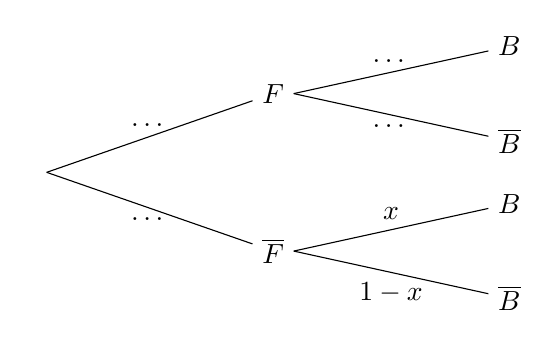
\begin{tikzpicture}[x=3cm, y=1cm]
			
			\node (root) at (0,0) {};
			\node (A) at (1,1) {$F$};
			\node (Abar) at (1,-1) {$\overline{F}$};
			\node (B1) at (2,1.6) {$B$};
			\node (B1b) at (2,0.4) {$\overline{B}$};
			\node (B2) at (2,-0.4) {$B$};
			\node (B2b) at (2,-1.6) {$\overline{B}$};
			
			\draw (root.east) -- (A) node[pos=0.5,above] {\ldots};
			\draw (root.east) -- (Abar) node[pos=0.5,below] {\ldots};
			
			\draw (A.east) -- (B1) node[pos=0.5,above] {\ldots};
			\draw (A.east) -- (B1b) node[pos=0.5,below] {\ldots};
			\draw (Abar.east) -- (B2) node[pos=0.5,above] {$x$};
			\draw (Abar.east) -- (B2b) node[pos=0.5,below] {$1-x$};
		\end{tikzpicture}
	\end{center}

	\item Montrer que la probabilité que le véhicule choisi soit un fourgon en bon état est égale à $0,3$.
	\item On sait que le véhicule choisi est en bon état. Déterminer la probabilité que ce soit un fourgon. On donnera le résultat sous la forme d'une fraction irréductible.
	\item Montrer que le réel $x$ est solution de l'équation $0,4x+0,3=0,66$.
	\item Résoudre l'équation et interpréter ce résultat dans le contexte de l'énoncé.
\end{enumerate}
